
\section{CIVIS Platform Design}

\subsection{Design Guidelines}

\subsection{CIVIS Platform Design}

The Improvement and Finalization 
\subsubsection{Action Suggestions}
\subsubsection{Housing Cooperatives}
Hammarby Sj�stad, Stockholm Test Site\\

\subsubsection{Energy Data Visualization and Comparison (need another title probably)}

Trento test site
%
%\info[inline]{
%
%A number of events for CIVIS design:
%
%-- CIVIS design workshop (Delft Nov. 2014) @Hanna: do you write this in D1.2? If so, we just need to have a ref here. 
%
%-- is there a focus group or other event in Stockholm?  @Hanna
%
%-- Helsinki Focus Group study (Helsinki June 2015) @Sanja
%
%-- Italian test site Focus Group study (Trentino Jul 2015) @Giacomo @
%
%-- others? 
%
%}


%need to find the sources: I've copied these from somewhere. 
%
%A basic idea in the CIVIS project is to engage users in the smart grid. 
%Survies and statistics show that despite many users are concerned about their energy use, and interested in reducing energy use and saving energy bill, little of them actually know what to do to achieve the goal. 
%Today, consumers still have a vague understanding of the power grid or what they can do with it. This is however very important, because how consumers understand the smart grid will shape how they feel about it, and in turn determines whether they are ready to use it, and how they use it. 
%
%To this end, it is very important how we present energy information (or information or knowledge of the power grid in general) to the users. 
%
%It is clear that we need to provide them with personalized information. And more importantly, we need to give them actionable information. 
%
%If consumers are given useful feedback on how they use energy, and they are given recommendations on how to improve, they will have the chances to make more informed energy choices. 
%
%This may have chances to yield crowdshifting effect, which simply means large-scale, voluntary behavioral change for social good. 
%
%There are many finer details in how to present users with information and how this could affect user behavior. All these are interesting topics to study. 

The side navigation (nav) is composed of six items, among which the ``Energy Data'' and ``Housing Cooperatives'' are activated respectively when a user authenticated his/her household's account for energy data (production is only for the Italian case) or when a user is a member of a housing cooperative (the Swedish case). Each tab item is associated with at least one view. Figure~\ref{fig:menu} shows an example: the ``Action List'' view of ``Your Actions'' tab with a closed (left) and an open (right) side navigation drawer. 

\begin{table}
\caption{YouPower app navigation structure}\label{tab:app_nav}
\begin{center} \footnotesize 
\begin{tabular}{ l l p{6cm}}
\hline
\textbf{Side Nav Items}  &
\textbf{Tab Items}  &
\textbf{Views}  \\ \hline

Actions & Your Actions & Action List, Action Suggestion, Action Details, Action Completed Form, Action Abandoned Form, etc.\\ 
& Household Actions & Member List, Action List, etc. \\ 
& Community Actions & Community List, Top Action List, Discussions, etc.\\ 
& Achievements & Achievement List (unlocked/locked), etc.\\  \hline

Energy Data  & Household Level  & Current Tarif (Trentino only), Current Consumption, Current Production, Historical Production/Consumption Patterns, Forecasted Tarifs (Trentino only)\\ 
& Appliance Level & Consumption Patterns (for each monitored appliance) \\ 
&  Community Level & Total Community Consumption (last month), Total Community Production (last month), Community Energy Balance, Comparison with Benchmark \\  \hline

Housing Cooperatives & Your Cooperative & Action List, Consumption per Category, Discussions, etc. \\ 
& Cooperatives in Neighborhood&  Action Map, Action List, Discussions, etc. \\  \hline

Donation (Trentino only) & n/a & Campaign Information, Campaign Status \\
\hline

Settings & Preferences & Form \\ 
& Personal Profile & Form \\ 
& Household Profile & Form, Eenergy Data Account \\  \hline

About & Q\&A & Q\&A List \\ 
& Help \& Feedback & Contact, Form\\ 
& Version Update & Version Info\\  \hline
\end{tabular}
\end{center} 
\end{table}

\begin{figure}
\begin{center}
	   \frame{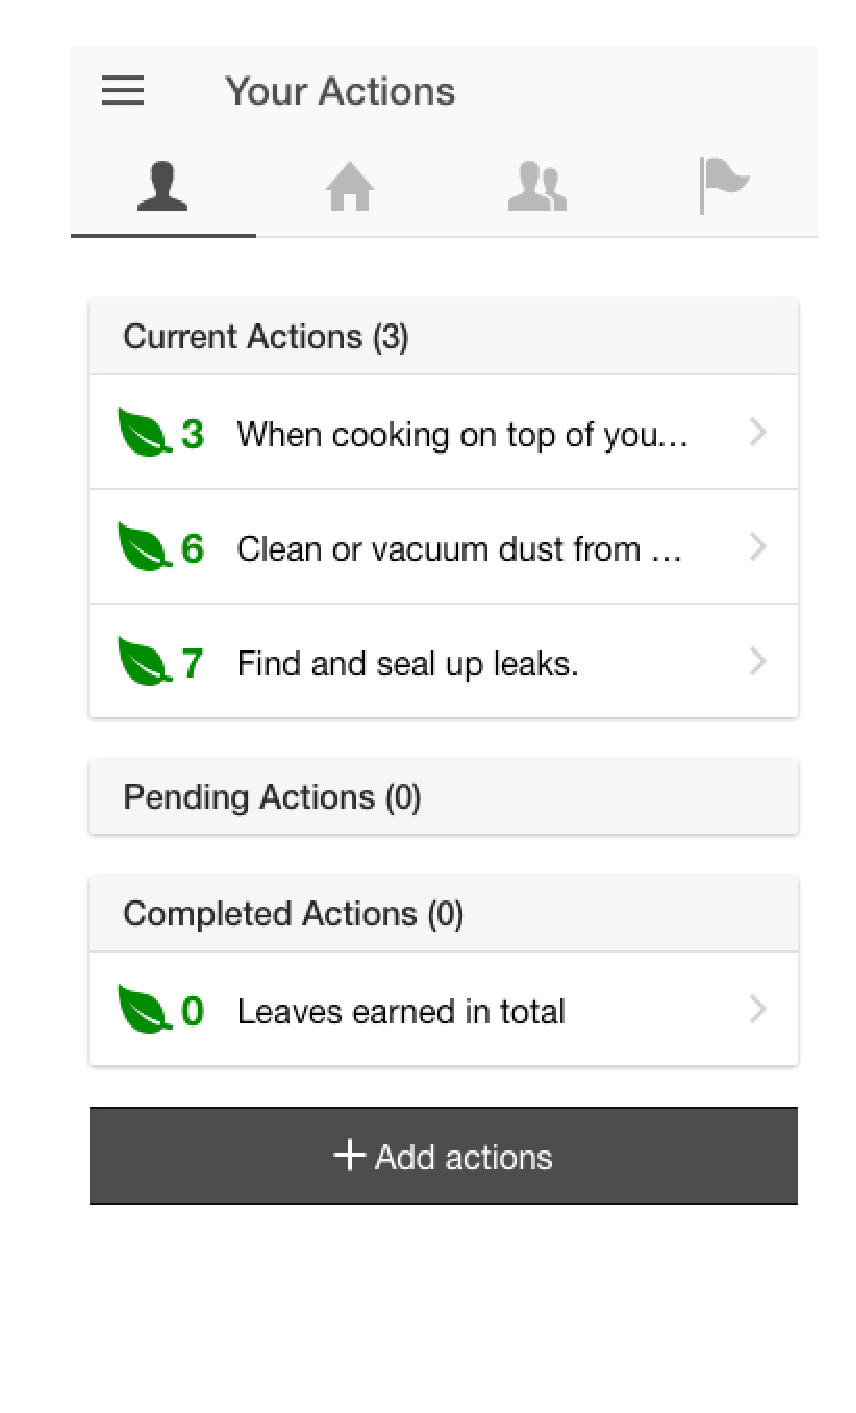
\includegraphics[height=0.55\textheight]{img/your_actions.pdf}}
		 \hfill
	   \frame{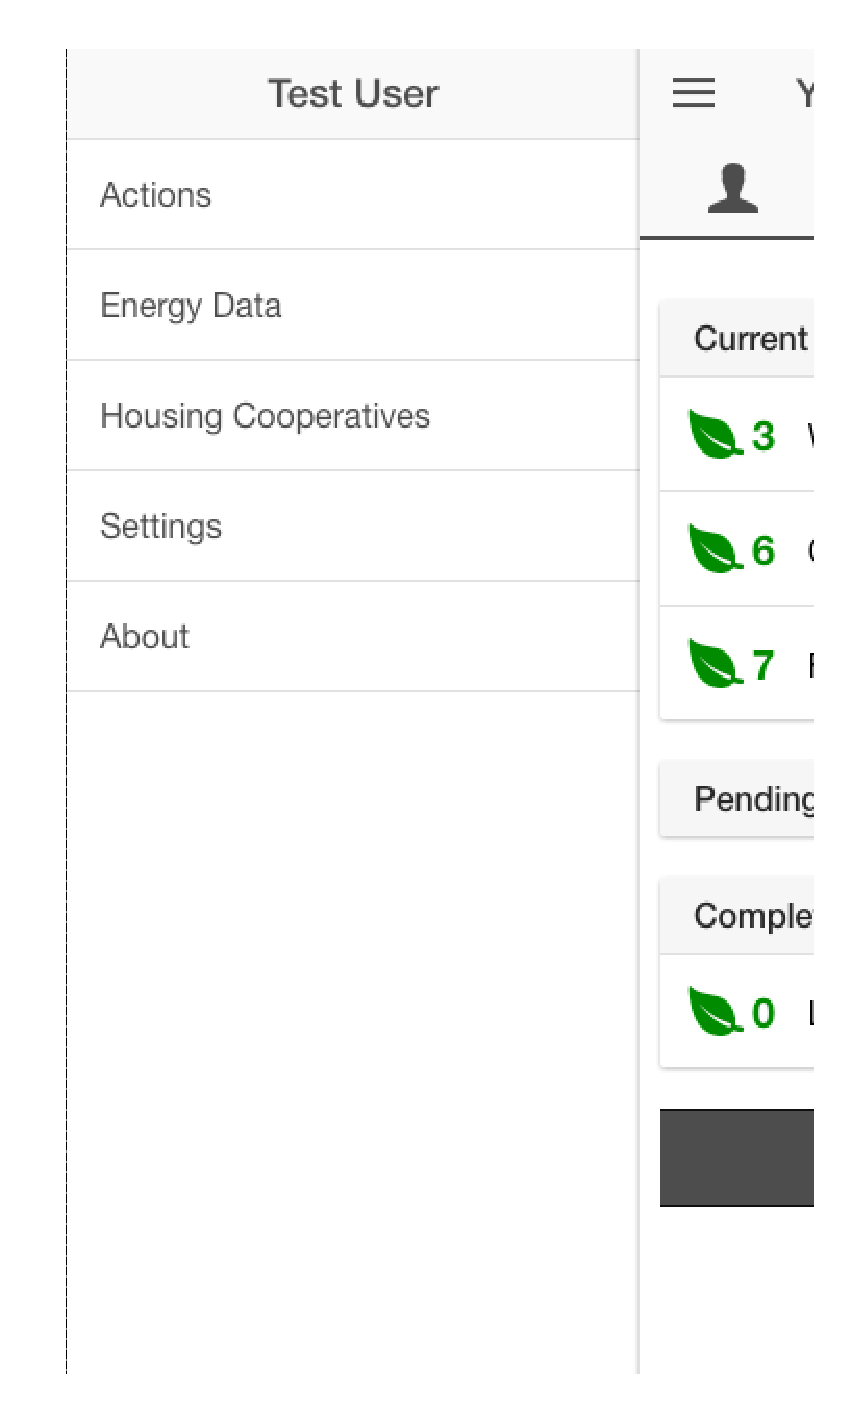
\includegraphics[height=0.55\textheight]{img/menu.pdf}}
	  \caption{``Your Actions'' tab -- ``Action List'' view (left); with an open side nav drawer (right)}\label{fig:menu}
\end{center}
\end{figure} 
The ``Action List'' is the index view of ``Your Actions'' tab. It is also the default view after user login. In this case, when the user presses on one of the ``Current Actions'', the app navigates to the ``Action Details'' view. Figure~\ref{fig:action_details} gives an example. 
% 
\begin{figure}
\begin{center}
	   \frame{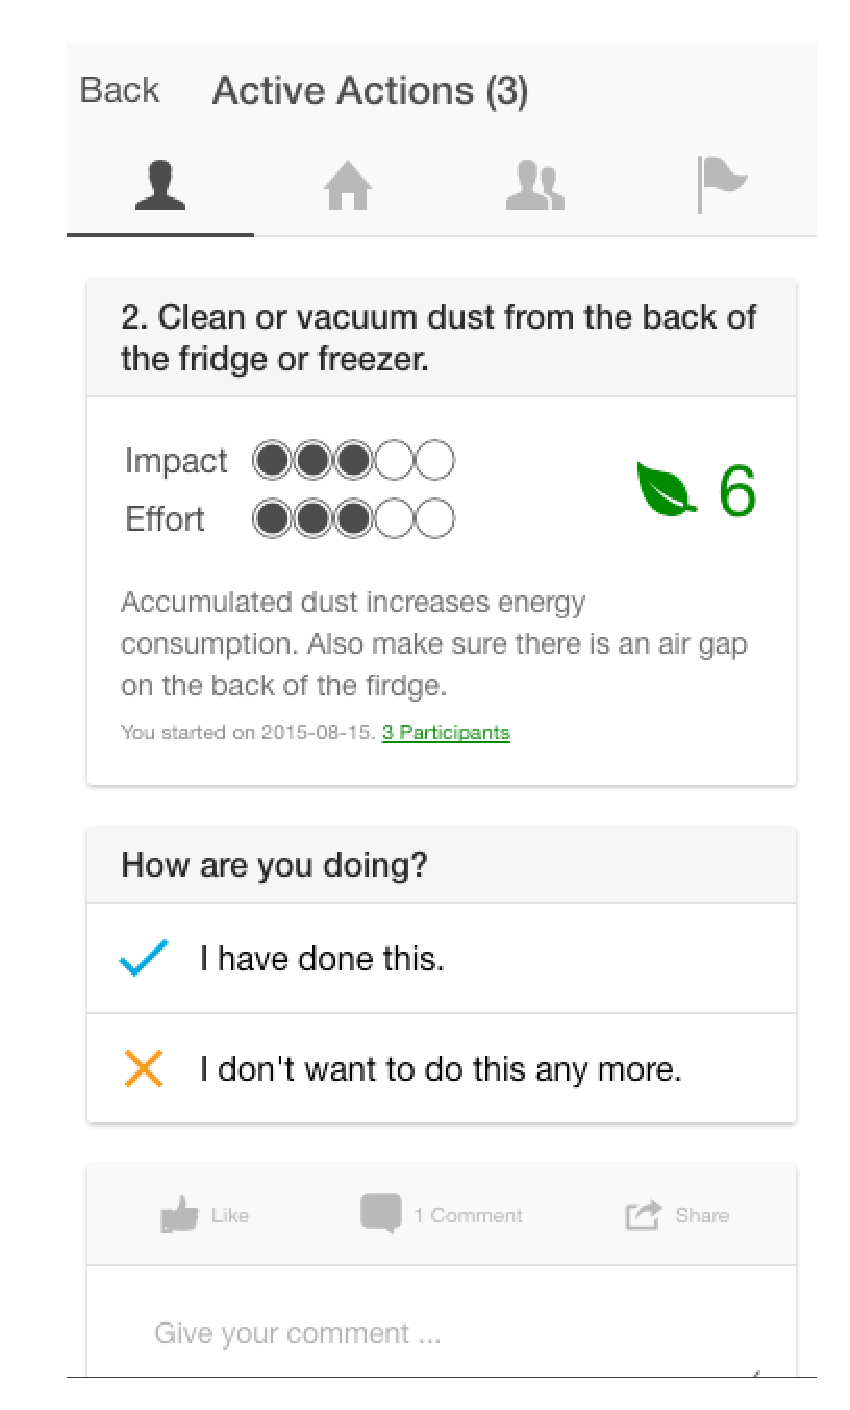
\includegraphics[height=0.55\textheight]{img/action_details.pdf}}\caption{``Your Actions'' tab -- ``Action Details'' view}\label{fig:action_details}
\end{center}
\end{figure} 
% 
